\documentclass[11pt,a4paper]{article}
\usepackage[T1]{fontenc}
\usepackage[utf8]{inputenc}
\usepackage{lmodern}
\usepackage[margin=1.05in,includefoot]{geometry}
\usepackage{microtype}
\usepackage{graphicx}
\usepackage{booktabs,tabularx,array}
\usepackage{caption}
\usepackage{enumitem}
\usepackage[section]{placeins}
\usepackage{multicol}
\usepackage{xurl}
\usepackage[unicode]{hyperref}
\input{glyphtounicode}
\pdfgentounicode=1
\hypersetup{hidelinks,pdfauthor={Felipe Sabino},pdftitle={Rehosting early iPhone OS on open mobile hardware: Native execution, hardware contracts and bounded acceptance},pdfsubject={Preprint prepared for arXiv submission; not yet submitted}}
\captionsetup{font=small,labelfont=bf,justification=raggedright,singlelinecheck=false}
\setlength{\emergencystretch}{2em}
\setlength{\parskip}{3pt}
\widowpenalty=10000
\clubpenalty=10000
\setlist{nosep,leftmargin=*}
\renewcommand{\topfraction}{0.9}
\renewcommand{\bottomfraction}{0.85}
\renewcommand{\textfraction}{0.08}
\renewcommand{\floatpagefraction}{0.7}
\title{Rehosting early iPhone OS on open mobile hardware: Native execution, hardware contracts and bounded acceptance}
\author{Felipe Sabino}
\date{7 October 2026}
\begin{document}
\maketitle
\begin{center}\small Preprint. Prepared for arXiv submission. Not yet submitted or peer reviewed.\end{center}
\begin{abstract}
Preserving a historical mobile operating system requires more than retaining its installation archive: observable behavior depends on obsolete processors, peripheral contracts and service ordering. This study investigates whether early iPhone OS can execute on an open, non-Apple mobile board while retaining original userspace consumers. We adapt the 1.1.4/4A102 and 3.1.3/7E18 kernels to the PinePhone's Allwinner A64 using shared original hardware adapters, kernel-hash-selected bindings and selective architectural compatibility handling. QEMU supplies bounded development gates; physical capture, protected-media readback and owner hand tests establish acceptance. The 7E18 daily trial accepts touch, battery indication, upright stock Camera preview, photo saving, complete power-off and reopening a photograph after cold power-on. Camera output is 1600 \(\times\) 1200, resampled from 640 \(\times\) 480 acquisition. A 64-presentation idle interval averages 12.7 ms of elapsed display work; a separate finite diagnostic reads 100 real accelerometer samples at 6.80 observed callbacks/s. Native USB enumeration and the stock mux handshake advance to a listener-readiness frontier, with ordinary pairing still pending. Case studies expose differences between modeled and physical CPU state, memory attributes, logging latency and inherited regulator ownership. The result is a bounded native preservation system and an auditable experimental method, rather than complete device compatibility or an independently reproducible public port. \hyperlink{e-E41}{\textsf{E41}} \hyperlink{e-E44}{\textsf{E44}} \hyperlink{e-E50}{\textsf{E50}} \hyperlink{e-E51}{\textsf{E51}} \hyperlink{e-E52}{\textsf{E52}} \hyperlink{e-E54}{\textsf{E54}} \hyperlink{e-E55}{\textsf{E55}}
\end{abstract}
\noindent\small\textbf{Publication boundary.} Edition 2.0; reviewed source snapshot
\texttt{15b3a95} (full revision in the ancillary data). AI-assisted investigation,
engineering and publication preparation; the author is responsible for the reviewed record.
The implementation, firmware and private experiment artifacts are not distributed.
Curated ancillary records support inspection, not independent public reproduction.
\normalsize
\section{Introduction}

Historical mobile software is unusually dependent on the device around it. A retained application may expect an old graphics service; that service may expect a particular kernel user client; the kernel may expect a processor instruction or power controller that no current board supplies. An archive preserves bytes. It does not, by itself, preserve the interaction among those layers.

This work asks a narrower, testable question: \textbf{can original early iPhone OS userspace operate through an adapted original kernel on an open mobile board, with hardware behavior accepted at named boundaries?} The native target is the original A64 PinePhone. The software targets are iPhone OS 1.1.4/4A102, with separate iPod touch and iPhone profiles, and iPhone OS 3.1.3/7E18 for the original iPhone. Their distinctions survive throughout the experiment. A shared historical kernel does not imply identical userspaces, peripheral expectations or acceptance. \hyperlink{e-E01}{\textsf{E01}} \hyperlink{e-E32}{\textsf{E32}} \hyperlink{e-E41}{\textsf{E41}}

``Native'' describes the ordinary instruction-execution path: AArch32 kernel and application instructions execute on the A64's Cortex-A53. The system still uses original replacement hardware providers and a resident compatibility/reset layer, including selective handling of legacy operations. It does not recreate the complete Apple board, and native execution does not imply an absence of traps or virtualization mechanisms. The partial PinePhone QEMU model is a separate development substrate. \hyperlink{e-E03}{\textsf{E03}} \hyperlink{e-E06}{\textsf{E06}} \hyperlink{e-E46}{\textsf{E46}}

The strongest current result is a physical 3.1.3 workflow. In the October 7 daily test, the owner unlocks the device, uses touch, sees battery and charging indication, blanks and wakes the display with Power, captures a photograph through the stock Camera app, opens it in Photos, powers the phone completely off and reopens the same photograph after cold power-on. This is useful preservation behavior, but it is not full phone functionality. Ordinary restart, networking, telephony, audio output, GPU acceleration, suspend and stock rotation retain separate open gates. \hyperlink{e-E51}{\textsf{E51}}

The study makes four contributions:

\begin{enumerate}

\item \textbf{A shared adaptation method across two historical builds.} Hardware algorithms remain shared while exact kernel identities select independently reviewed object layouts, method bindings and entry contracts.

\item \textbf{A bounded physical system with stock consumers.} Display, input, storage, power and Camera reach real device behavior without changing the accepted 3.1.3 Apple userland instructions or relaxing signature checks.

\item \textbf{An experimental acceptance method.} Frozen staging, finite trials, recovery, immutable-region hashing, fresh filesystem checks and owner hand tests separate progress from acceptance.

\item \textbf{Discriminating failures and measured boundaries.} The paper retains model/hardware disagreements, rejected approaches and instrument limitations alongside timing, camera and USB results. \hyperlink{e-E41}{\textsf{E41}} \hyperlink{e-E44}{\textsf{E44}} \hyperlink{e-E47}{\textsf{E47}} \hyperlink{e-E50}{\textsf{E50}} \hyperlink{e-E53}{\textsf{E53}}

\end{enumerate}

This is a versioned research publication derived from private experiments. The evidence pages publish selected fields, reviewed captures and original explanations. They identify the unavailable source reports by basename, digest and locator. That supports an authorized audit; it does not provide independent public reproduction. The claims ledger exposes the claim-to-source mapping, and the edition note fixes the October 7 boundary.

\begin{figure}[htbp]
\centering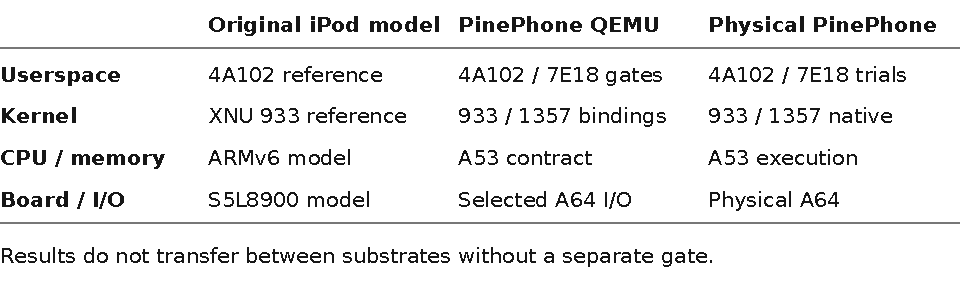
\includegraphics[width=\linewidth]{figures/substrates.pdf}
\caption{Distinct execution substrates. Original print schematic separating the
4A102 iPod reference, partial PinePhone QEMU contract and physical 4A102/7E18
results. This is explanatory organization, not a measured call graph.}
\label{fig:1}\end{figure}

\section{Background}

\subsection{The boards and software builds}

The original iPhone and first-generation iPod touch targets belong to the S5L8900/ARM11 generation. The PinePhone instead supplies an Allwinner A64 with Cortex-A53 cores, a GIC, eMMC, a 720 \(\times\) 1440 panel, a Goodix touch controller, an AXP803 power-management device, an OV5640 rear sensor and MUSB USB hardware. The public board description establishes available hardware; it does not establish that the native XNU port drives each peripheral. In particular, the PinePhone has an EG25-G modem even though native telephony integration is unaccepted. \cite{ref-1} \cite{ref-2} \hyperlink{e-E32}{\textsf{E32}}

The inspected 4A102 kernel identifies XNU 933.0.0.211, while 7E18 identifies XNU 1357.5.30. Both selected historical kernels are ARM32, but their boot arguments, reserved initialization space, service layouts and userspace contracts differ. Public XNU source explains architectural organization; a nearby release is not proof of either proprietary ARM binary's layout. The source inspection and exact-build binding gates carry that burden. \cite{ref-3} \hyperlink{e-E27}{\textsf{E27}} \hyperlink{e-E41}{\textsf{E41}}

\begin{table}[htbp]
\centering
\caption[]{The two accepted software generations are not interchangeable ABIs. The kernel identities come from reviewed target inspection; original-root differences and shared 4A102 kernel identity are separate observations. \hyperlink{e-E01}{\textsf{E01}} \hyperlink{e-E41}{\textsf{E41}}}
\small\setlength{\tabcolsep}{4pt}\renewcommand{\arraystretch}{1.18}
\begin{tabularx}{\linewidth}{@{}>{\raggedright\arraybackslash}X>{\raggedright\arraybackslash}X>{\raggedright\arraybackslash}X@{}}
\toprule
\textbf{Software target} & \textbf{Original product context} & \textbf{Kernel identity / adaptation boundary} \\
\midrule
1.1.4 / 4A102 & N45AP iPod touch and M68AP iPhone; separate roots & XNU 933.0.0.211; retained older binding and memory-layout contract \\
3.1.3 / 7E18 & M68AP / iPhone1,1 & XNU 1357.5.30; independently measured bindings, IOSurface and newer service expectations \\
\bottomrule
\end{tabularx}
\end{table}

\subsection{XNU and IOKit contracts}

XNU combines Mach, BSD and IOKit. Mach supplies tasks, threads and messaging; BSD supplies process and filesystem behavior; IOKit organizes C++ services, provider matching and device clients. Applications rarely need to know which physical controller ultimately performs a request. They do need the expected service to publish, accept a correctly shaped method, preserve ownership and complete honestly. Apple's architecture description provides this context. \cite{ref-3} \cite{ref-4}

A replacement provider is therefore more than a plausible register driver. Storage has completion status and byte-count obligations; graphics has surface mapping and retirement; Camera has descriptors, dimensions, color ranges and asynchronous completion; HID has stable contact identities. Service registration proves discovery at one boundary. It cannot prove successful application use. \hyperlink{e-E09}{\textsf{E09}} \hyperlink{e-E10}{\textsf{E10}} \hyperlink{e-E15}{\textsf{E15}} \hyperlink{e-E29}{\textsf{E29}} \hyperlink{e-E44}{\textsf{E44}}

\subsection{Boot time and runtime are different layers}

The firmware handoff supplies initial CPU, memory and peripheral state. In the current SD-free route, Tow-Boot resides in the eMMC hardware boot area. A pre-XNU NuttX initializer and selector prepare the panel and choose a profile; the selected AArch32 XNU then owns the running OS. NuttX is boot-time preparation, not a Linux host underneath iPhone OS. The resident EL2 compatibility/reset path has a different lifetime from that initializer. Jumpdrive is the separate Linux recovery environment entered after a reset. \hyperlink{e-E43}{\textsf{E43}} \hyperlink{e-E46}{\textsf{E46}} \hyperlink{e-E48}{\textsf{E48}} \hyperlink{e-E61}{\textsf{E61}}

The inherited state is not an empty board. Regulators, clock gates, muxes and DMA-related fields may already belong to another boot stage. A native provider must verify its prerequisites, acquire only what it owns and preserve unrelated fields. The Tow-Boot/SD U-Boot comparison later in this paper shows why one assumed reset baseline was insufficient. \hyperlink{e-E49}{\textsf{E49}}

\section{Related work}

\textbf{Whole-system emulation and virtualization.} QEMU-iOS models early iPod touch hardware and provides an essential reference for historical behavior. Aleph Security's iOS-on-QEMU work targets later iOS, documents QEMU/KVM execution and exposes an intentionally altered debugging/security configuration. Their board models and research acceptance are not the physical PinePhone contracts established here. \cite{ref-5} \cite{ref-6}

Corellium uses ARM-native virtualization through its CHARM hypervisor. It should not be described as instruction-by-instruction CPU emulation. Its virtual mobile-device platform shares the concern of supplying device contracts, but the present study addresses a specific physical open phone, historical AArch32 builds and owner-visible peripheral acceptance. No performance or capability comparison with Corellium was run. \cite{ref-7}

\textbf{Preservation at other boundaries.} touchHLE preserves early iOS applications through high-level emulation rather than booting the historical kernel and original service stack. Legacy iOS Kit supports restoration and related work on original Apple devices. It is relevant to preservation practice, but its firmware-patching route was not used for the accepted local-activation path here. Project Sandcastle takes the reverse direction, bringing Android/Linux to iPhone hardware. These approaches preserve different units: application behavior, original devices, or an alternative OS on an existing board. \cite{ref-8} \cite{ref-9} \cite{ref-10}

\textbf{Open mobile hardware.} PINE64 documentation, the mainline PinePhone device tree and the postmarketOS ecosystem provide hardware and Linux-port context. Those sources help identify components and ownership expectations; Linux support does not automatically transfer into IOKit. The postmarketOS device page was inaccessible to the review fetch after a redirect and anti-bot response, so this paper makes no current support claim from that page. Readable PINE64 documentation and the pinned mainline description support the board facts. \cite{ref-1} \cite{ref-2} \cite{ref-11}

\textbf{Translation and rehosting literature.} Bellard describes QEMU's portable dynamic translation and full-system emulation. Avatar combines emulation with real embedded hardware for analysis, while P2IM abstracts peripheral interfaces to make firmware testing progress without the original hardware. These works show why CPU execution and peripheral behavior must be considered separately. Our engineering distinction is physical acceptance: a modeled return value can advance a test while failing to establish a real display, radio or power transition. \cite{ref-12} \cite{ref-13} \cite{ref-14}

The resulting position is specific, without a priority claim: \textbf{native execution of selected historical iPhone OS builds on a physical non-Apple mobile board, using original hardware providers and explicitly bounded evidence}. Neither the literature review nor the private experiments establish that this is the first such execution in all historical settings.

\section{System design}

\begin{figure}[htbp]
\centering
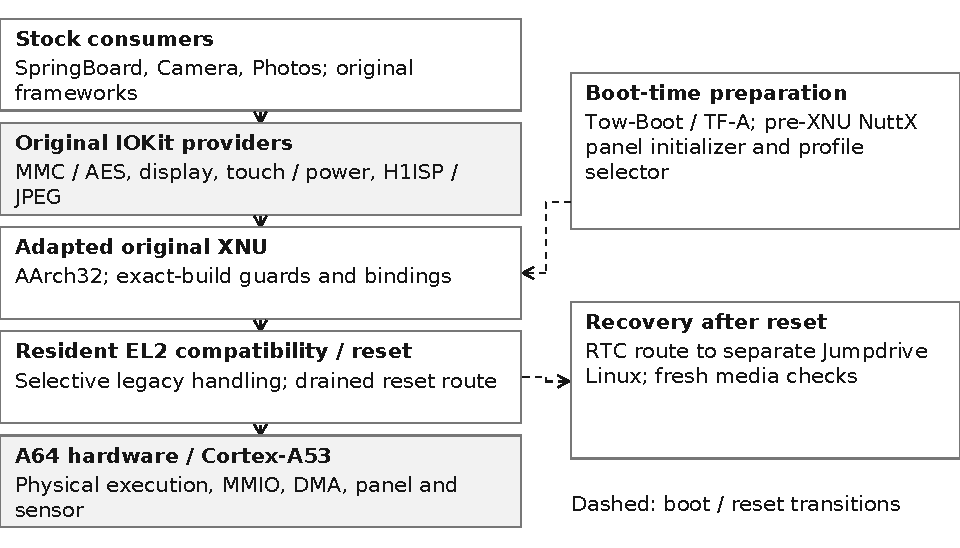
\includegraphics[width=\linewidth]{figures/native-architecture.pdf}
\caption[]{\textbf{Boot and runtime architecture.} Original schematic for the 7E18 PinePhone route. NuttX performs boot-time panel/selector work; ordinary kernel and application instructions execute as AArch32 on the A53. Original providers supply hardware contracts beneath stock consumers. Resident EL2 compatibility/reset and separate Jumpdrive recovery are distinct branches. This is explanatory organization, not a captured call graph. \hyperlink{e-E41}{\textsf{E41}}, \hyperlink{e-E46}{\textsf{E46}}, \hyperlink{e-E48}{\textsf{E48}}.}
\label{fig:2}
\end{figure}

\subsection{Exact identity before adaptation}

An input kernel digest selects a reviewed binding contract. Unknown content or a conflicting build name is rejected. Bindings include object fields, method slots, callback instruction state and callable targets. Guards check the expected original context before an intervention is admitted. This reduces a dangerous failure mode: treating two similar releases as one ABI and interpreting a valid pointer through the wrong layout. \hyperlink{e-E41}{\textsf{E41}}

The shared implementation retains A64 hardware algorithms across 4A102 and 7E18. Separate binding data expresses the differences. Storage completion, queue backpressure and explicit-key AES behavior need not be forked merely because an inherited method table changes. Conversely, sharing source is not evidence that every binding is correct. Each build must pass its own admission and client gates.

\subsection{Adapt a contract, preserve its failures}

Guarded hooks replace hardware-facing behavior where the original platform cannot perform it. They are not a policy of making every unsupported operation return success. Unknown instructions retain their original exception fallback; unsupported camera/USB operations remain unsupported; signing failures remain failures. Progress is useful only if the new result represents the requested operation. \hyperlink{e-E06}{\textsf{E06}} \hyperlink{e-E44}{\textsf{E44}} \hyperlink{e-E52}{\textsf{E52}}

The display supplies software-rendered stock surfaces rather than pretending to provide the original GPU. The camera supplies sensor-derived buffers and a kernel JPEG endpoint rather than modifying signed Apple userland to force a save. Local activation uses an already present stock branch, narrowly scoped to its measured caller; unrelated identity queries retain their stock purpose. Those choices preserve the distinction between an original client working through a new provider and a client whose checks have been disabled. \hyperlink{e-E43}{\textsf{E43}} \hyperlink{e-E44}{\textsf{E44}}

\subsection{Reserve memory and storage ownership explicitly}

Native providers require memory outside the ordinary allocator, alongside translation tables, graphics pools and scanout. The 7E18 reservation plan gives growing providers separate slots and moves the allocation frontier only after checking the complete layout. A retained rejected trial exposed an old cold-entry guard that still expected the earlier table frontier. Reservation metadata and loaded code therefore form one contract. \hyperlink{e-E41}{\textsf{E41}}

Disk ownership is independently bounded. Separate OS windows prevent one profile from silently writing another. The boot partition's growth preserves the OS payloads and uses reserved GPT entries to prevent those windows from being mistaken for free space. A boot-time memory address is not a disk interval, and neither reservation can substitute for the other. \hyperlink{e-E47}{\textsf{E47}}

\section{Implementation}

\subsection{CPU, translation and legacy synchronization}

The A53 executes the historical ARM instruction stream, but privileged startup cannot assume ARM1176-specific registers or cache geometry. The adaptation handles exercised incompatibilities through reviewed cold-entry, MMU and cache policy, while rejecting unexpected state. Translation must account for descriptor interpretation as well as backing memory: an earlier A53 access-flag control rejected a legacy descriptor despite valid physical backing. A matched change in interpretation advanced the commpage read. \hyperlink{e-E03}{\textsf{E03}} \hyperlink{e-E04}{\textsf{E04}} \hyperlink{e-E05}{\textsf{E05}} \hyperlink{e-E42}{\textsf{E42}}

Legacy SWP instructions require exchange semantics, not merely a skipped opcode. The physical startup path records handled exchanges and subsequent progress. A separate 4A102 hotspot change greatly reduces observed traps, but its measured UI frame gaps do not improve consistently. Complete atomicity, fault handling, copy-on-write and multiprocessor semantics remain wider obligations than the accepted workload. \hyperlink{e-E06}{\textsf{E06}} \hyperlink{e-E39}{\textsf{E39}}

\subsection{Timer and interrupt delivery}

Original kernel scheduling needs a real timebase and interrupts through the expected callback path. Native A64 timer/GIC work replaces the original controller interface; counter units remain explicit. A timer count proves that callbacks execute, not that userspace remains healthy. Diagnostic watchdog petting is finite and independent of normal profiles. The sensor and display measurements use the nominal 24 MHz counter, with their measurement boundary attached. \hyperlink{e-E07}{\textsf{E07}} \hyperlink{e-E08}{\textsf{E08}} \hyperlink{e-E40}{\textsf{E40}} \hyperlink{e-E50}{\textsf{E50}} \hyperlink{e-E55}{\textsf{E55}}

\subsection{Storage, AES and service order}

The original storage family receives real queue and completion behavior from the A64 MMC provider. Request bounds, byte counts, register preservation, asynchronous ownership, backpressure and final drain matter as much as sector bytes. Historical completion failures demonstrate why a visible block device is insufficient. Read-only root policy, RAM-only diagnostic data and permitted persistent private-data writes are separately declared. \hyperlink{e-E10}{\textsf{E10}} \hyperlink{e-E11}{\textsf{E11}} \hyperlink{e-E13}{\textsf{E13}} \hyperlink{e-E14}{\textsf{E14}}

For 7E18, the shared software AES provider supplies explicit-key operations and rejects nonzero UID/GID selections. It does not recreate hardware-bound device keys or a modern keybag. Stock file-integrity startup remains in the service order; bringing required providers up correctly resolves the dependency without changing the integrity policy. Later daily persistence is established by actual fresh media readback and hand use, rather than inherited from an earlier QEMU mount. \hyperlink{e-E41}{\textsf{E41}} \hyperlink{e-E51}{\textsf{E51}}

\subsection{Display and stock software composition}

The display provider must publish under the expected service parent, expose the correct surface contract and retire submissions. In the initial 7E18 route, a display completion counter coexisted with repeated SpringBoard crashes in the hardware compositor. The selected stock software-renderer path removes that unavailable GPU dependency through ordinary launch configuration; it does not change Apple executable instructions. Captured QEMU guest pixels then show the English lock/home transition. Physical scanout and later human use are separate gates. \hyperlink{e-E43}{\textsf{E43}}

The original 320 \(\times\) 480 interface is doubled to 640 \(\times\) 960 and centered within the 720 \(\times\) 1440 panel. This is a bounded copy/expansion route, not a full-panel rescale or GPU driver. Surface backing, task permissions, source aliases and device visibility remain separate questions. The idle timing experiment measures this route without changing its cache or clock policy. \hyperlink{e-E15}{\textsf{E15}} \hyperlink{e-E17}{\textsf{E17}} \hyperlink{e-E50}{\textsf{E50}}

\subsection{Input, local activation and locale}

Goodix contacts reach the original Z2 multitouch consumer through the native input adapter. Home/Power events traverse the original HID path. Packet delivery and visible gestures require separate checks: the October 3 7E18 physical replay used synthetic contacts; the October 7 daily hand test establishes human touch. The earlier 4A102 work also shows that two contact records with one interpreted identity cannot prove pinch. \hyperlink{e-E29}{\textsf{E29}} \hyperlink{e-E43}{\textsf{E43}} \hyperlink{e-E51}{\textsf{E51}}

The local activation path uses a stock lockdownd branch whose hardware query receives the synthetic research response only at the measured activation caller. No Apple/carrier service is contacted, and signing/FairPlay policy is unchanged. Broadly scoping an identity response to the entire daemon would affect other queries with different meanings. English preferences belong to the private data configuration. São Paulo time-zone installation and libc/CoreFoundation resolution pass their checks, but the owner-visible clock check is still pending. \hyperlink{e-E43}{\textsf{E43}} \hyperlink{e-E54}{\textsf{E54}} \hyperlink{e-E62}{\textsf{E62}}

\subsection{Power, halt and restart}

Battery values originate in the physical PMIC and publish through the expected power-source service. A charging icon is an accepted UI observation, not a battery-endurance result. Older measurements show why input budget and workload matter: blanking and a bright lock screen produce different battery balances under the recorded USB limit. Power blank/wake also does not establish system suspend. \hyperlink{e-E31}{\textsf{E31}} \hyperlink{e-E51}{\textsf{E51}}

Clean halt follows stock shutdown through cleanup, sync/unmount and final native storage drain before bounded PMIC power-off. Earlier camera restoration failures are retained and must block shutdown rather than be suppressed. Continuous capture records the corrected Power-slider route; the daily test confirms that the phone stays off before cold power-on. \hyperlink{e-E45}{\textsf{E45}} \hyperlink{e-E51}{\textsf{E51}}

Restart exposes another boundary. The TF-A HVC/PSCI route stalls, including the diagnostic version-query path. The accepted single confirmation instead enters qualified EL2 after drain and resets with WDOG0, reaching a new SPL and the ordinary selector. This proves that route once. It does not close repeated ordinary stock-restart hand acceptance. Normal boot/runtime watchdogs remain off; a final post-drain reset fallback is a distinct safety mechanism. \hyperlink{e-E46}{\textsf{E46}}

\subsection{Camera and JPEG}

The accepted 7E18 path is stock PhotoLibrary \(\rightarrow\) Celestial/FigRecorder \(\rightarrow\) H1ISP/IOSurface consumers, supplied by original kernel camera and JPEG providers. Real OV5640/CSI acquisition produces 640 \(\times\) 480 UYVY. The provider delivers the expected preview and still formats, uses bounded destination ownership and keeps the exclusive CSI ring separate. The kernel encoder serves the stock AppleJPEGDriver user client. Apple userland instructions and signature checks remain unchanged in this clean route. \hyperlink{e-E44}{\textsf{E44}}

The 1600 \(\times\) 1200 still is resampled from that VGA acquisition. It satisfies the stock format contract but adds no captured scene detail. Owner acceptance covers preview, shutter, thumbnail, Photos and persistence. The first successful hand test lacks contemporaneous UART, and its pre-reboot JPEG digest was not extracted. We therefore report reopening and decoded post-reboot media, not byte-identical before/after persistence for that test. The later daily trial supplies continuous UART and cold-power-cycle acceptance. \hyperlink{e-E44}{\textsf{E44}} \hyperlink{e-E51}{\textsf{E51}}

\begin{figure}[htbp]
\centering
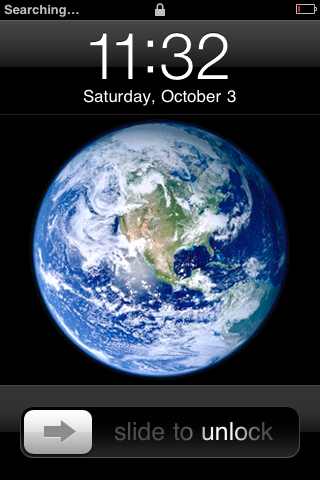
\includegraphics[width=.31\linewidth]{figures/E43-313-lock-qemu.png}
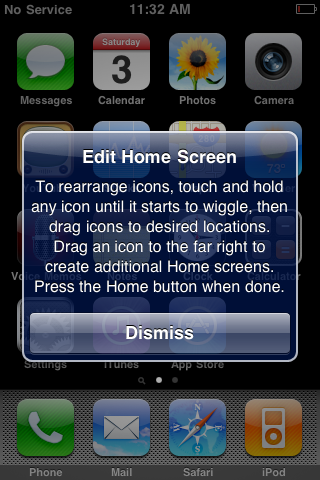
\includegraphics[width=.31\linewidth]{figures/E43-313-home-qemu.png}
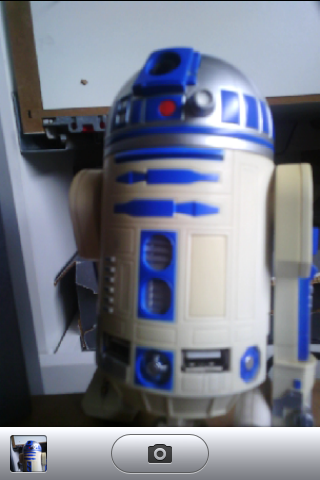
\includegraphics[width=.31\linewidth]{figures/E44-313-camera-stock.png}
\caption[]{\textbf{Genuine captures from distinct experiments.} Left and middle: 7E18 guest pixels before and after synthetic unlock/Home replay in QEMU; the stock home-screen overlay is preserved. Right: an unmodified stock Camera screenshot recovered from physical private-data storage. All selected files retain original bytes and pixels, with source basenames and SHA-256 in \hyperlink{e-E43}{\textsf{E43}} and \hyperlink{e-E44}{\textsf{E44}}. None is a photograph of the panel, and the cellular labels establish no radio connection.}
\label{fig:3}
\end{figure}

\subsection{Selector, eMMC and recovery}

The physical panel selector defaults after twelve seconds and accepts Volume/Power navigation in its separately reviewed back-buffer trial. Bounded damage copies replace unnecessary direct redraws. Later title/background styling remains a separate candidate; the accepted controls cannot certify that candidate's visual behavior. The publication has no reviewed selector panel photograph and uses the architecture schematic rather than manufacturing one. \hyperlink{e-E43}{\textsf{E43}} \hyperlink{e-E61}{\textsf{E61}}

AHVBOOT growth and reserved GPT entries prepare boot space without moving or overwriting OS windows. The SD-free route uses the existing eMMC bootloader, the selector and Jumpdrive; the installation does not rewrite that bootloader. RTC recovery state is consumed before profile entry, and explicit trial profiles retain finite watchdog paths. The deliberate early-stall test never reaches XNU, so its fast return cannot be attributed to guest shutdown. \hyperlink{e-E47}{\textsf{E47}} \hyperlink{e-E48}{\textsf{E48}}

\subsection{USB and finite sensors}

The original MUSB provider operates beneath stock IOUSBDeviceFamily. Admission covers the actual full-speed PTP+Mux configuration, endpoint/FIFO ownership, pending request completion and real controller state. EP0 address and configuration failures precede later enumeration and bulk work; their traces remain useful rather than being replaced by the final milestone. The passed stock mux handshake advances to local BSD connect and listener timing, with ordinary pairing and services pending. \hyperlink{e-E52}{\textsf{E52}} \hyperlink{e-E53}{\textsf{E53}} \hyperlink{e-E54}{\textsf{E54}} \hyperlink{e-E60}{\textsf{E60}}

A separate MPU6050 diagnostic admits its live memory mapping before touching the bus, reads a finite sequence and restores owned MPU/TWI state. It is not installed as a stock motion provider. A sibling shutdown test establishes one cleanup route through frozen-code inference and its observed success continuation; it does not prove callback join or unloading. Raw measurements must not be promoted to automatic screen rotation. \hyperlink{e-E55}{\textsf{E55}} \hyperlink{e-E56}{\textsf{E56}}

\section{Methodology and safety}

\subsection{The trial is the unit of acceptance}

Each trial declares its build, loaded profile, substrate, writable scope, capture method and recovery path. Staging verifies the frozen inputs before boot. QEMU checks exercised control flow, bounded fixtures and regression gates before a physical run, but does not certify physical cache attributes, regulator state, USB timing or power transitions. \hyperlink{e-E13}{\textsf{E13}} \hyperlink{e-E26}{\textsf{E26}} \hyperlink{e-E49}{\textsf{E49}}

The physical loop is stage \(\rightarrow\) boot \(\rightarrow\) capture \(\rightarrow\) recovery \(\rightarrow\) readback. Exclusive UART ownership avoids concurrent readers or accidental commands. Host-side USB observations, device RAM traces and counter timestamps retain distinct clocks and completeness limits. Watchdog/RTC recovery is finite for diagnostic profiles; it is not silently enabled in accepted daily profiles. Owner hand tests run only after the necessary technical gate and provide a different form of evidence from automated capture. \hyperlink{e-E40}{\textsf{E40}} \hyperlink{e-E48}{\textsf{E48}} \hyperlink{e-E51}{\textsf{E51}} \hyperlink{e-E54}{\textsf{E54}}

\begin{figure}[htbp]
\centering
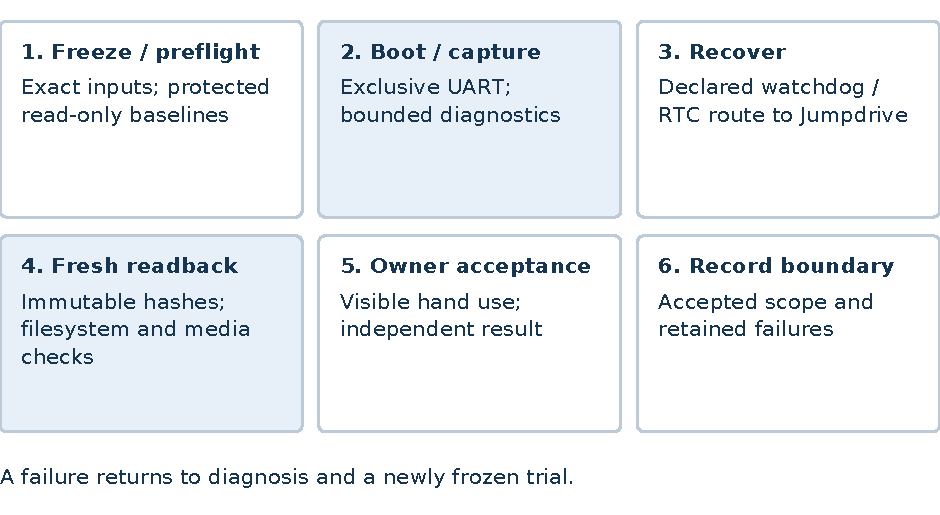
\includegraphics[width=\linewidth]{figures/trial-loop.pdf}
\caption[]{\textbf{Bounded experimental loop.} Original schematic of the physical 7E18 method. Diagnostic watchdog leases and RTC return are configured per trial; accepted normal profiles keep boot/runtime watchdogs disabled. Protected bytes, permitted private-data deltas and owner-visible behavior are separate acceptance gates. A failed gate remains in the record and returns to diagnosis. \hyperlink{e-E48}{\textsf{E48}}, \hyperlink{e-E51}{\textsf{E51}}, \hyperlink{e-E54}{\textsf{E54}}.}
\label{fig:4}
\end{figure}

\FloatBarrier

\subsection{Integrity checks after recovery}

The host re-reads available protected intervals and staged files after execution, then compares immutable content with its baseline. Permitted private-data changes are assessed separately with fresh root/data copies, filesystem checks and decoded media. A ``passed'' run summary cannot replace these postconditions. Absent SD media are reported as absent, not counted as re-read. Recovery Linux's clean filesystem state is not automatically the guest's clean shutdown state. \hyperlink{e-E47}{\textsf{E47}} \hyperlink{e-E48}{\textsf{E48}} \hyperlink{e-E51}{\textsf{E51}}

Earlier camera recovery required a narrowly bounded private-data repair after a failed shutdown. That history is preserved beside the later clean halt. It prevents a misleading claim that every successful photograph was followed by an initially clean data volume. Likewise, finite USB cancellation can retain references until reset rather than prove complete teardown. \hyperlink{e-E44}{\textsf{E44}} \hyperlink{e-E45}{\textsf{E45}} \hyperlink{e-E52}{\textsf{E52}}

\subsection{Two axes of evidence}

\begin{table}[htbp]
\centering
\caption[]{Evidence classification has both a substrate and an observation method. ``In progress'' is an acceptance state, not a sixth substrate. Mixed records identify which part belongs to which environment. Claims ledger, research method.}
\small\setlength{\tabcolsep}{4pt}\renewcommand{\arraystretch}{1.18}
\begin{tabularx}{\linewidth}{@{}>{\raggedright\arraybackslash}X>{\raggedright\arraybackslash}X>{\raggedright\arraybackslash}X>{\raggedright\arraybackslash}X@{}}
\toprule
\textbf{Substrate} & \textbf{Method} & \textbf{What the method can establish} & \textbf{What it cannot inherit} \\
\midrule
Original iPod model & Reference capture/replay & Modeled original-client behavior & Physical Apple or PinePhone behavior \\
Partial PinePhone QEMU & Guest trace, fixture, snapshot & Executed adapter/client gate in that model & Real MMIO attributes, electrical state or panel use \\
Physical PinePhone & UART, counter, host protocol capture, readback & Named runtime events and post-run bytes & Human usability or unobserved wire-level ACKs \\
Physical PinePhone & Owner hand test & The reported visible interaction in that profile & Every app, performance, durability or missing trace \\
Files/binaries & Static inspection & Exact inspected layouts or control flow & Runtime completion or responsive UI \\
Synthetic probe & Purpose-built fixture & The isolated contract under supplied assumptions & Complete client lifetime or real hardware \\
\bottomrule
\end{tabularx}
\end{table}

\section{Evaluation}

The evaluation addresses four questions: does the shared design reach original consumers across builds; which physical interactions are accepted; what do the measurements actually count; and what remains after the latest USB gate? The corpus is one evolving project on one physical phone, not a benchmark population. The following tables select named experiments without constructing an aggregate success rate from overlapping reports.

\subsection{Boot and visible acceptance}

The October 3 default-selector trial provides buffered host-receipt milestones. The difference between the menu-start and choice markers is 12.049 seconds, consistent with the intended twelve-second selection. The later display and launchd markers are stages in that run, not universal cold-boot latencies. The run's synthetic touch replay is superseded only for human use by the separate daily hand test. \hyperlink{e-E43}{\textsf{E43}} \hyperlink{e-E51}{\textsf{E51}}

\begin{table}[htbp]
\centering
\caption[]{One physical 7E18 selector trial, measured from its host capture origin. UART buffering and work before each printed marker limit timing interpretation. Source: \texttt{pinephone-iphone313-stage4-selector-2026-10-03.json}, \texttt{/selector\_physical\_run/markers\_seconds}. \hyperlink{e-E43}{\textsf{E43}}}
\small\setlength{\tabcolsep}{4pt}\renewcommand{\arraystretch}{1.18}
\begin{tabularx}{\linewidth}{@{}>{\raggedright\arraybackslash}X>{\raggedright\arraybackslash}X>{\raggedright\arraybackslash}X@{}}
\toprule
\textbf{Milestone} & \textbf{Host receipt, s} & \textbf{Interpretation} \\
\midrule
Selector menu starts & 6.587 & Pre-XNU selector marker \\
Default 3.1.3 choice & 18.636 & 12.049 s after menu marker \\
Display route & 23.687 & Native pipeline marker; no panel photograph in this run \\
launchd & 44.974 & Stock userspace milestone \\
Jumpdrive recovery & 204.703 & Diagnostic return, not ordinary interactive reboot latency \\
\bottomrule
\end{tabularx}
\end{table}

The October 7 daily test is stronger for end-to-end use: accepted touch and Camera behavior coincide with continuous UART and fresh available-region recovery. Power-slider shutdown stays off for thirty seconds, then cold power-on reopens the new photograph. Ordinary restart is explicitly outside that acceptance. \hyperlink{e-E51}{\textsf{E51}}

\subsection{Camera throughput and output detail}

The historical 1.1.4 comparison changes queue capacity from two to six. Different native-delivery, renderer-selection and panel-update rates reveal the bottleneck: panel updates can repeatedly reuse one selected image. The comparison improves distinct selection while native delivery falls modestly. It is one physical pair with unequal intervals, not a controlled multi-run speed claim and not a 3.1.3 measurement. \hyperlink{e-E59}{\textsf{E59}}

\begin{table}[htbp]
\centering
\caption[]{Physical legacy Camera comparison from \texttt{/controlled\_phone\_comparison/phone13} and \texttt{/phone14}. ``Selected'' is the original renderer boundary; these counters do not individually prove physical panel presentation. Unequal sampling windows and one pair limit generalization. \hyperlink{e-E59}{\textsf{E59}}}
\small\setlength{\tabcolsep}{4pt}\renewcommand{\arraystretch}{1.18}
\begin{tabularx}{\linewidth}{@{}>{\raggedright\arraybackslash}X>{\raggedright\arraybackslash}X>{\raggedright\arraybackslash}X>{\raggedright\arraybackslash}X@{}}
\toprule
\textbf{1.1.4 preview queue} & \textbf{Native deliveries/s} & \textbf{Distinct selected images/s} & \textbf{Panel update counter/s} \\
\midrule
Two slots, before first still & 29.621 & 7.893 & 30.210 \\
Six slots, early steady preview & 26.279 & 16.520 & 30.544 \\
\bottomrule
\end{tabularx}
\end{table}

\begin{figure}[htbp]
\centering
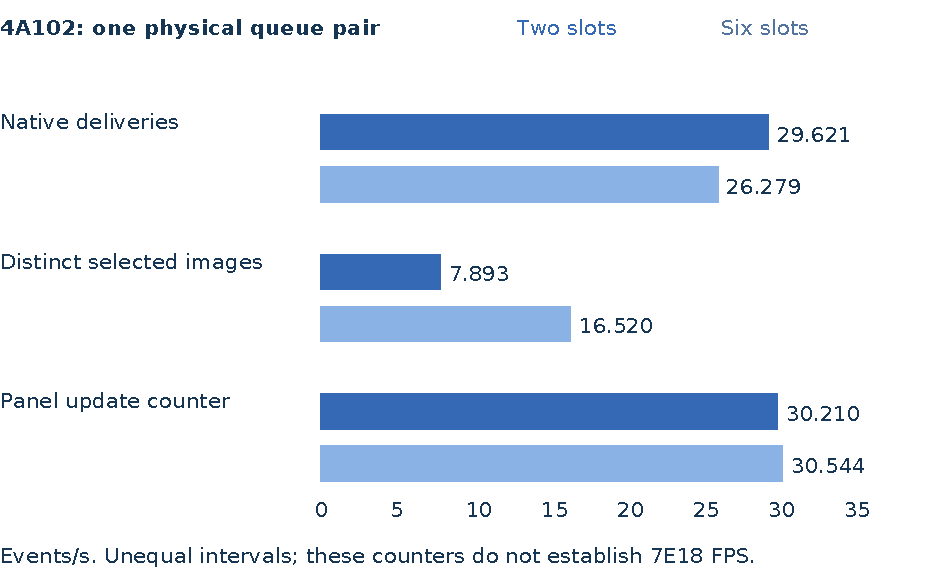
\includegraphics[width=\linewidth]{figures/camera-rates.pdf}
\caption[]{\textbf{More updates do not imply more distinct camera images.} Original plot of one physical 4A102 queue comparison. Each rate counts the boundary named beside its bars. The native-delivery, selected-image and update samples are not interchangeable; the pair has unequal intervals. These values are not measured 7E18 preview throughput. \hyperlink{e-E59}{\textsf{E59}}.}
\label{fig:5}
\end{figure}

\begin{table}[htbp]
\centering
\caption[]{7E18 output geometry is a stock-client contract, not evidence of 1600 \(\times\) 1200 acquisition. The first successful Camera hand test has a UART gap and no pre-reboot JPEG digest. The daily test is a separate later result. \hyperlink{e-E44}{\textsf{E44}} \hyperlink{e-E51}{\textsf{E51}}}
\small\setlength{\tabcolsep}{4pt}\renewcommand{\arraystretch}{1.18}
\begin{tabularx}{\linewidth}{@{}>{\raggedright\arraybackslash}X>{\raggedright\arraybackslash}X>{\raggedright\arraybackslash}X@{}}
\toprule
\textbf{3.1.3 Camera boundary} & \textbf{Recorded format} & \textbf{Accepted scope} \\
\midrule
Actual sensor acquisition & 640 \(\times\) 480 UYVY, full range & Real sensor-derived source \\
Stock preview destination & 400 \(\times\) 304 YUYV, video range & Upright preview accepted by owner \\
Stock still destination/output & 1600 \(\times\) 1200; resampled source, JPEG output & Save, thumbnail and Photos accepted; no extra captured detail \\
After power cycle & Same new photo opens in Photos & Daily cold-power-cycle acceptance; broader durability unproven \\
\bottomrule
\end{tabularx}
\end{table}

\FloatBarrier

\subsection{Display elapsed-time baseline}

The later 64-presentation interval contains zero sampled source changes. Its mean total cost is 12.6937 ms, dominated by source work and expansion. The presentation gap is 12.8638 ms. These are elapsed counter observations around an idle route, which can include interruption and scheduling effects. They do not yield an animation frame rate or pure compositor CPU utilization. \hyperlink{e-E50}{\textsf{E50}}

\begin{table}[htbp]
\centering
\caption[]{Physical 7E18, presentations 64-exclusive through 128-inclusive, nominal 24 MHz counter, zero sampled changes. Component means are instrumented boundaries and are not asserted to partition every tick exactly. Cache policy and CPU clock are unchanged. The single logging sample is not a 64-frame average. \hyperlink{e-E50}{\textsf{E50}}}
\small\setlength{\tabcolsep}{4pt}\renewcommand{\arraystretch}{1.18}
\begin{tabularx}{\linewidth}{@{}>{\raggedright\arraybackslash}X>{\raggedright\arraybackslash}X>{\raggedright\arraybackslash}X@{}}
\toprule
\textbf{Instrumented boundary} & \textbf{Samples} & \textbf{Mean elapsed ms} \\
\midrule
Source work & 64 & 4.7924 \\
2\(\times\) expansion & 64 & 7.8142 \\
Synchronization & 64 & 0.0004 \\
Completion & 64 & 0.0382 \\
Total work & 64 & 12.6937 \\
Presentation gap & 64 & 12.8638 \\
Diagnostic log & 1 & 72.3972 \\
\bottomrule
\end{tabularx}
\end{table}

\begin{figure}[htbp]
\centering
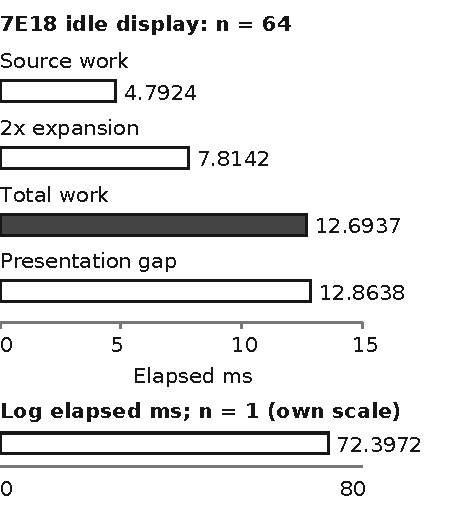
\includegraphics[width=\linewidth]{figures/display-timing.pdf}
\caption[]{\textbf{Idle presentation cost and instrumentation cost.} Original plot of the later 64-presentation physical 7E18 interval. The upper bars share a millisecond scale; the log is explicitly a separate single sample. Zero sampled changes make this an idle baseline. It is not an animation benchmark or a cache-policy comparison. \hyperlink{e-E50}{\textsf{E50}}.}
\label{fig:6}
\end{figure}

\FloatBarrier

\subsection{USB protocol ladder}

USB success is a sequence of gates. Real bus reset and descriptor transfer precede address application; full configuration precedes bulk mux traffic; mux framing precedes a local listener connection; ordinary pairing precedes service access. A later trial stays enumerated, records three stock mux reads and three writes without mux I/O errors, and passes the host v2 handshake. Finite cleanup still returns BUSY and retains prerequisites until reset. \hyperlink{e-E52}{\textsf{E52}}

\begin{table}[htbp]
\centering
\caption[]{The latest state combines distinct dated experiments rather than pretending one capture proves every gate. Complete matched mux frames are narrower evidence than whole-usbmon completeness, which remains false. \hyperlink{e-E52}{\textsf{E52}} \hyperlink{e-E53}{\textsf{E53}} \hyperlink{e-E54}{\textsf{E54}} \hyperlink{e-E60}{\textsf{E60}}}
\small\setlength{\tabcolsep}{4pt}\renewcommand{\arraystretch}{1.18}
\begin{tabularx}{\linewidth}{@{}>{\raggedright\arraybackslash}X>{\raggedright\arraybackslash}X>{\raggedright\arraybackslash}X@{}}
\toprule
\textbf{Gate} & \textbf{Reported state at this edition} & \textbf{Remaining qualification} \\
\midrule
EP0 descriptor/address & Passed in later quiet/protocol trials & Earlier address and stale-DATAEND failures retained \\
Native host enumeration & Passed in later finite physical trial & Repeated replug/general endurance pending \\
Stock usbmux v2 handshake & Passed & Does not imply pairing \\
Local lockdownd connection & Earlier complete frames receive ECONNREFUSED/RST & Listener readiness and host preflight ordering \\
TCP listener census & First positive sample 41.237 s after daemon startup & Not exact bind time or an implemented listener gate \\
Ordinary pairing / info / syslog / AFC & Pending & Actual service acceptance and two-boot identity stability \\
\bottomrule
\end{tabularx}
\end{table}

\begin{figure}[htbp]
\centering
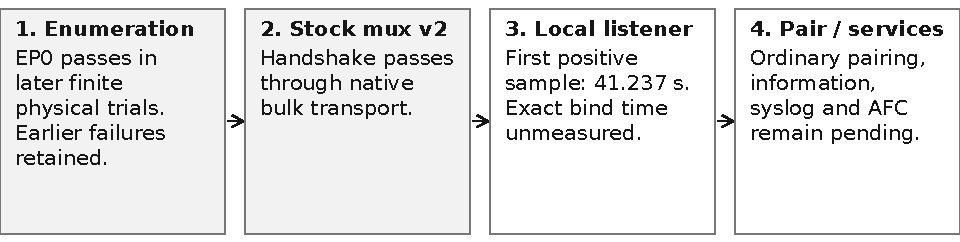
\includegraphics[width=\linewidth]{figures/usb-ladder.pdf}
\caption[]{\textbf{The current USB frontier is a service-readiness boundary.} Original schematic of physical 7E18 progress. Passed enumeration and mux gates do not promote the sampled listener into accepted ordinary pairing. The latest diagnostic has scoped success and verified recovery while its original whole-run completeness gate remains false. \hyperlink{e-E52}{\textsf{E52}}, \hyperlink{e-E54}{\textsf{E54}}.}
\label{fig:7}
\end{figure}

The combined listener diagnostic enumerates at host receipt 83.705 s and returns automatically to Jumpdrive at 248.893 s. Twenty-five periodic samples retain the first observed listener and genuine CommCenter check-in. Its original runner remains false because capture ownership/completion and bounded-head marker gates are incomplete. No application-level pairing success is inferred from the successful recovery. \hyperlink{e-E54}{\textsf{E54}}

\FloatBarrier

\subsection{Recovery, integrity and sensor diagnostics}

\begin{table}[htbp]
\centering
\caption[]{Selected recovery and integrity reports, not an aggregate reliability percentage. Origins differ and are named explicitly. The RTC-only trial's timing and the separately recorded SD-free integrity check are not one fabricated continuous run. Absent SD intervals are not re-read. \hyperlink{e-E46}{\textsf{E46}} \hyperlink{e-E48}{\textsf{E48}} \hyperlink{e-E51}{\textsf{E51}} \hyperlink{e-E54}{\textsf{E54}} \hyperlink{e-E55}{\textsf{E55}} \hyperlink{e-E56}{\textsf{E56}}}
\small\setlength{\tabcolsep}{4pt}\renewcommand{\arraystretch}{1.18}
\begin{tabularx}{\linewidth}{@{}>{\raggedright\arraybackslash}X>{\raggedright\arraybackslash}X>{\raggedright\arraybackslash}X>{\raggedright\arraybackslash}X@{}}
\toprule
\textbf{Named physical trial} & \textbf{Recovery / transition, s} & \textbf{Reported checked scope} & \textbf{Result / limit} \\
\midrule
Pre-XNU RTC-only stall & 23.287 to Jumpdrive & SD-free recovery separately checks 12 regions, 218 files & XNU never starts; deliberate early-stall route \\
Finite sensor stream & 154.018 to Jumpdrive & 12 checked intervals, 11 immutable; 575 staged files & Immutable bytes match; finite restoration \\
Sensor shutdown sibling & 78.210 to Jumpdrive & 12 checked intervals, 11 immutable; 593 staged files & Stock drain and unique success continuation; no join/unload proof \\
Daily owner test & Not reported as a timed recovery benchmark & 12 available intervals; 593 boot files; fresh root/data fsck exit 0 & Permitted private-data changes; other protected content preserved \\
Combined listener diagnostic & 248.893 to Jumpdrive & 12 regions; 793 staged files & Protected bytes match; original whole-run/capture gate false \\
Direct EL2 reset confirmation & 1.084 EL2 \(\rightarrow\) new SPL & Separate clean-volume/protected readback & One reset confirmation; ordinary repeatability pending \\
\bottomrule
\end{tabularx}
\end{table}

The finite sensor stream records 100 samples across 14.562433 s, with an observed callback rate of 6.7983 Hz and mean axes approximately (0.041482, 0.006206, 1.026641) g. This is raw sampling in one stationary configuration, not calibrated orientation or measured hardware output data rate. No stock motion publication or owner rotation acceptance follows from these numbers. \hyperlink{e-E55}{\textsf{E55}}

\FloatBarrier

\subsection{Milestone chronology}

\begin{table}[htbp]
\centering
\caption[]{Commit subjects locate the engineering chronology in the pinned private corpus; validation records support the results. A commit date alone does not prove acceptance. Earlier milestones and their original publication snapshots remain in the research timeline.}
\small\setlength{\tabcolsep}{4pt}\renewcommand{\arraystretch}{1.18}
\begin{tabularx}{\linewidth}{@{}>{\raggedright\arraybackslash}X>{\raggedright\arraybackslash}X>{\raggedright\arraybackslash}X>{\raggedright\arraybackslash}X@{}}
\toprule
\textbf{Date} & \textbf{Reviewed milestone} & \textbf{Source commit} & \textbf{Evidence} \\
\midrule
1 Oct & Physical legacy Camera queue comparison & \texttt{2cd7963} & E59 \\
2 Oct & Shared storage/AES and headless 7E18 userspace & \texttt{1258eb0}, \texttt{7cca234} & E41-E42 \\
3 Oct & Physical userspace, stock software UI and selector & \texttt{336a454}, \texttt{1680566}, \texttt{fc8269d} & E43 \\
4 Oct & Clean stock Camera/Photos and persistence & \texttt{c408727}, \texttt{0ebb304} & E44 \\
5 Oct & Accepted halt, direct EL2 reset, stable selector & \texttt{969b530}, \texttt{8760690}, \texttt{d970afa} & E45-E46, E61 \\
6 Oct & AHVBOOT growth and SD-free recovery & \texttt{0f98ebe}, \texttt{ea66db4} & E47-E48 \\
7 Oct & Daily hand test, finite sensors and timing baseline & \texttt{0daf16b}, \texttt{7b1f989}, \texttt{967ee0a}, \texttt{1b759d0} & E50-E51, E55-E56 \\
7 Oct & USB enumeration/mux, then sampled listener frontier & \texttt{2bf60c6}, \texttt{df891b1}, \texttt{15b3a95} & E52, E54 \\
\bottomrule
\end{tabularx}
\end{table}

\section{Case studies: useful disagreements and failures}

\subsection{A too-strict HCR check, then stale linkage}

The cold-entry contract originally expected a modeled HCR state. Physical A53 readback retains SWIO as a RES1 bit. Correcting the admission rule to account for that physical value, while rejecting other unexpected HCR bits, addresses a hardware/model difference without broadly relaxing CPU policy. A zero-only test would reject valid physical state. \hyperlink{e-E42}{\textsf{E42}}

The next failure had a different cause. Relinking CPU helpers moved two functions while the SWP module retained old direct branch destinations. A physical candidate reached launchd and then panicked. Rebuilding the linkage against the actual loaded CPU object corrected those calls. The lesson is that a semantic fix can invalidate a placement assumption: admission must verify the complete loaded closure, not just the newly edited function. The source chapter preserves the failed candidate and repair; no binary patch recipe is published. \hyperlink{e-E42}{\textsf{E42}}

\subsection{An odd checksum address and a compiler-combined STRH}

The original Z2 packet writer places a trailing checksum after a variable-length body. That can make the checksum address odd. The October 3 committed rationale records that XNU enables alignment faults and that the compiler can combine adjacent writes into an unaligned halfword store. Keeping the checksum as explicit byte stores preserves the intended packet bytes without disabling alignment checks. C62

This is a deliberately bounded case study. The available chapter/validation corpus does not provide a standalone matched QEMU-versus-hardware exception receipt for this incident. We do not invent a fault PC, exception count or elapsed time. The source/commit establishes the implementation reason; later accepted touch establishes the combined path, not every possible alignment case. That distinction is itself part of the reporting method.

\subsection{SWP progress is not complete atomicity or a UI multiplier}

An old exchange instruction can repeatedly trap on a newer core while the rest of startup looks healthy. Handling the exchange advances the observed original workload. Skipping it would substitute different synchronization semantics. The bounded accepted case still leaves faults, permissions, copy-on-write and concurrency as explicit wider questions. \hyperlink{e-E06}{\textsf{E06}}

A paired hotspot replay subsequently reduces mean legacy atomic traps by 98.50-99.91\% across its interaction windows. Yet mean frame gaps improve in two windows and worsen in two. A local overhead reduction therefore cannot be presented as a comparable UI speedup. Instrumented trap counts answer a different question from application latency. \hyperlink{e-E39}{\textsf{E39}}

\subsection{eMMC MMIO needs the right memory attributes}

An early physical MMC clock update times out while the adapter uses the late mapping result directly. Remapping the two controller pages through a non-cacheable descriptor path advances the physical failure to a different controller condition. A translated address and successful mapping call were not sufficient evidence of device-access semantics. The next rejected assumption required a mode bit that the A64 eMMC controller does not implement. \hyperlink{e-E63}{\textsf{E63}}

This history is not a measured CPU-clock optimization. It is a correction to the device contract, followed by another actual hardware distinction. QEMU's ability to advance through register accesses cannot establish the physical memory attribute or implemented controller feature.

\subsection{SET\_ADDRESS timing and UART instrumentation}

USB requires applying the device address after genuine status completion and soon enough for the host's next addressed transaction. USB 2.0 §9.2.6.3 permits a 2 ms recovery interval after that status stage; controller ownership cannot be replaced with a fabricated completion. Synchronous UART printing on this path can occupy the same scarce service time as EP0. The quiet control preserves protocol/MMIO behavior while reducing hot-path logging. \cite{ref-15} \hyperlink{e-E60}{\textsf{E60}}

The quiet trial applies and verifies FADDR 1.136083 ms after the status command; stock address dispatch takes 8.917 \(\mu\)s, and the host receives the addressed 18-byte descriptor. This supports logging as a latency contributor. It does not measure the status-IRQ-to-FADDR latency or prove that logging caused every failure. The next configuration request instead exposes stale DATAEND retained across STALL/new SETUP, where a strict guard rejects the state before loading configuration bytes. A timing improvement reveals a second protocol bug; it does not justify weakening the guard. \hyperlink{e-E60}{\textsf{E60}}

\subsection{The caller of an identity query matters}

The stock local-activation branch and the daemon's ordinary hardware classification both query machine identity. Returning the synthetic activation response to every query in the same process conflates their purposes. The accepted policy narrows the special response to the measured activation caller and leaves the primary classification query with its stock answer. Signed text and unrelated queries remain unchanged. \hyperlink{e-E43}{\textsf{E43}} \hyperlink{e-E54}{\textsf{E54}}

The later listener diagnostic also separates a running process from an accepting socket. lockdownd remains alive, and CommCenter performs a genuine check-in with sampled run-loop activity. Those observations provide no basis to invent an absent-baseband shim or declare pairing accepted. Process existence, initialization state and listener readiness are different gates.

\subsection{Tow-Boot has already enabled a camera rail}

The initial camera admission assumed a quiescent regulator baseline. Tow-Boot's inherited state already programs and enables the analog rail at 2.8 V, while the digital supply starts off. The earlier policy rejects that state even though it is a legitimate prerequisite for the new route. The revised 7E18 policy verifies and adopts the supported state, normalizes only owned fields, quiesces CSI/DMA and restores masked ownership. \hyperlink{e-E49}{\textsf{E49}}

Two identical snapshot programs compare the eMMC Tow-Boot and SD U-Boot handoffs. Twenty-six changed records are reported, but battery/SD conditions also differ and five gated display words remain unavailable. Programmed voltage selectors are not voltage measurements. The result supports explicit handoff admission; it does not prove that every difference is caused by the bootloader. Exact 4A102 camera bindings retain their separate acceptance policy.

\subsection{A fixed delay is not listener readiness}

The fixed-delay USB trial waits a measured 30.0155 s before soft-connect and still receives genuine local ECONNREFUSED/RST. It falsifies the sufficiency of that candidate. The source's earlier broad timing interpretation is retained; it should not be rewritten into a retrospectively obvious success. \hyperlink{e-E53}{\textsf{E53}}

The later diagnostic first positively samples the TCP listener 41.237 s after daemon startup, while the host preflight starts earlier at attach. This supports readiness ordering as a new explanation, but the first positive sample is not the exact bind time. The activation log interval is not isolated RSA cost. A listener-gated connection is a next candidate beyond this committed publication snapshot; ordinary pairing is still pending. \hyperlink{e-E54}{\textsf{E54}}

There is a second negative result: an earlier kernel snapshot reaches its parent deadline without automatic recovery and needs owner reset. Later diagnostic recovery succeeds and verifies protected media, but cannot erase that failed return. The combined latest capture still has unknown host ownership and missing completion identities, so scoped diagnostic success must coexist with a false original whole-run gate. \hyperlink{e-E54}{\textsf{E54}}

\section{Discussion and threats to validity}

\textbf{A partial system.} The daily workflow is a substantial endpoint, but broad application coverage, GPU/GLES compatibility, audible output, Wi-Fi/Bluetooth, telephony, full suspend, motion-driven rotation and higher-detail sensor modes are not established. No Service is not proof of missing modem hardware, and an idle CPU is not proof of charging or low whole-system power. The public capability status keeps these limits beside accepted features. \hyperlink{e-E31}{\textsf{E31}} \hyperlink{e-E32}{\textsf{E32}} \hyperlink{e-E51}{\textsf{E51}} \hyperlink{e-E55}{\textsf{E55}}

\textbf{Small and evolving sample.} Physical measurements come from one phone and a small number of named trials. Legacy camera queue windows differ in duration and startup context. The direct reset result is one confirmation. The display interval is idle and instrumented. No random order, multi-device variance, broad app benchmark or general uptime distribution is claimed. The recorded values are useful for identifying the next bottleneck, not estimating a population effect. \hyperlink{e-E46}{\textsf{E46}} \hyperlink{e-E50}{\textsf{E50}} \hyperlink{e-E59}{\textsf{E59}}

\textbf{The observer can change the result.} UART output is buffered for host timing and can disturb a USB hot path. A 1 ms timer request is not guaranteed callback cadence. Logging's display sample is much larger than the idle work mean. Device RAM observations, host URBs and wire-stage ACKs are not equivalent views. A zero dropped-event counter cannot compensate for unassigned ownership or missing completion identity. \hyperlink{e-E50}{\textsf{E50}} \hyperlink{e-E54}{\textsf{E54}} \hyperlink{e-E60}{\textsf{E60}}

\textbf{Static inference and owner reports.} Frozen code plus a unique observed continuation can support one cleanup-route inference without proving join/unload. The first successful Camera test has owner evidence and readback but no contemporaneous UART, and no pre-reboot JPEG digest supports byte identity. Later continuous-capture daily acceptance improves that coverage without retrospectively supplying the missing earlier trace. \hyperlink{e-E44}{\textsf{E44}} \hyperlink{e-E51}{\textsf{E51}} \hyperlink{e-E56}{\textsf{E56}}

\textbf{Selection and publication limits.} The curated corpus is an author-reviewed record of private experiments. It is not peer review, an external replication or a complete public artifact package. Document hashes establish identity of the material reviewed, not the truth of unavailable contents. Source chapters can lag later validation; the ledger retains the more specific dated gate rather than treating the README or an old status row as uniformly current. Negative results remain visible to reduce success-only reporting.

\section{Ethics and publication boundary}

The experiments use the owner's hardware and isolated research profiles. Synthetic research identities are kept separate from real device identities. The accepted local workflow does not contact Apple/carrier activation services, bypass signing/FairPlay or decrypt another device's UID-bound private data. These are technical scope statements drawn from the reviewed experiments; they are not legal conclusions about every jurisdiction or potential redistribution. \hyperlink{e-E41}{\textsf{E41}} \hyperlink{e-E43}{\textsf{E43}} \hyperlink{e-E44}{\textsf{E44}} \hyperlink{e-E57}{\textsf{E57}}

This repository distributes original writing, diagrams, curated data organization and website code. It does not distribute firmware, keys, Apple implementation code, binary patches, storage images, raw sessions, credentials or private identifiers. Selected research captures retain provenance and unchanged pixels. Depicted third-party interfaces and subjects retain their original rights; MIT applies only to the repository's original contributions. Apple names identify the software descriptively. This publication is independent and is not an Apple or PINE64 product.

AI agents assisted investigation, adapter engineering, test development and publication preparation. Their suggestions and generated prose are not experiment results. Felipe Sabino is the author responsible for the hardware work, selected publication record and its review. Claims remain tied to captures, validation and hand acceptance rather than agent confidence.

\section{Future work}

The immediate connectivity path is USB service acceptance: measure/admit listener readiness, complete ordinary private pairing, retrieve version information, sustain syslog and retrieve a saved photo over AFC with a verified hash. Replug, cancellation and lifetime behavior remain required. Only then should a stock USB-network function or a declared original CDC-ECM route establish bidirectional local traffic. Wi-Fi adds SDIO, power ownership and an exact IO80211 contract; it does not follow automatically from USB enumeration. No cellular-state fabrication is a substitute for those gates. \hyperlink{e-E52}{\textsf{E52}} \hyperlink{e-E54}{\textsf{E54}} \hyperlink{e-E57}{\textsf{E57}}

Motion work needs signed-axis calibration, lifetime admission, real stock HID publication and owner-visible rotation. Performance work needs matched moving-UI trials and measurements of application latency, source/expansion cost and still/JPEG cost. Genuine higher-detail sensor acquisition must precede a higher-resolution quality claim. Repeatable ordinary restart acceptance is separate from cold-power-cycle persistence. \hyperlink{e-E44}{\textsf{E44}} \hyperlink{e-E46}{\textsf{E46}} \hyperlink{e-E50}{\textsf{E50}} \hyperlink{e-E55}{\textsf{E55}}

\begin{table}[htbp]
\centering
\caption[]{Conditional engineering ranking, not accepted ports or measured effort. Selected kernels' 4 KiB page geometry does not establish CPU/MMU or service compatibility. The inspected 5s userland renderer does not independently validate the iPhone 6 renderer. \hyperlink{e-E57}{\textsf{E57}} \hyperlink{e-E58}{\textsf{E58}}}
\small\setlength{\tabcolsep}{4pt}\renewcommand{\arraystretch}{1.18}
\begin{tabularx}{\linewidth}{@{}>{\raggedright\arraybackslash}X>{\raggedright\arraybackslash}X>{\raggedright\arraybackslash}X@{}}
\toprule
\textbf{Ranked prospective target} & \textbf{Evidence at this edition} & \textbf{Main new gate} \\
\midrule
1. 3GS iOS 6.1.6 / 10B500 & Offline study; separate diskless QEMU work reaches CPUIdle and two-input dispatch, then clock-gate panic & Exact newer bindings, authentic normal boot, fresh keybag lifecycle and physical display \\
2. iPhone 5 iOS 10.3.4 / 14G61 & Static software-renderer route and ARM32 inspection & New service/keybag contracts, larger isolated storage layout and runtime fallback \\
3. iPhone 5s / 6 iOS 12.5.7 / 16H81 & ARM64/kernel inspection; 5s renderer inspected separately & Original AArch64 platform and SEP-dependent service contracts; no fake-key shortcut \\
\bottomrule
\end{tabularx}
\end{table}

The latest 10B500 QEMU work deserves a precise frontier: actual host press/release stimuli reach preserved stock keyboard dispatch and CPUIdle setup, then an absent function-clock\_gate dependency panics. No authentic normal Darwin banner, root, launchd, stock reset, graphical session or physical boot is accepted. Static feasibility and this partial runtime gate are separate studies. \hyperlink{e-E58}{\textsf{E58}}

\section{Reproducibility appendix}

\subsection{What a public reader can inspect}

The publication repository contains the paper, companion summary, chapter atlas, original schematics, selected captured fields/images, references, claims ledger and generated portable edition. The structured index and claim export preserve the editorial layer in ordinary JSON. Each evidence page links an inspectable excerpt and source identity. Its underlying complete private report and implementation are unavailable here.

An authorized independent hardware audit would require the matching licensed historical software inputs, reviewed private implementation, original A64 PinePhone, the declared eMMC/profile layout, UART/host capture equipment and verified recovery/backups. Public hardware and architecture references are necessary context but cannot reconstruct exact private bindings from their names. This paper is therefore a partial reproducibility artifact: the publication can be rebuilt and its exported claim graph checked; the native port cannot be reproduced solely from this repository.

\subsection{Record an experiment without importing it}

The record identity contains a committed source revision, source basename, SHA-256 and exact JSON pointer or selected passage locator. The report states substrate, method, inputs/control, observation, permitted mutations, recovery postconditions and remaining gates. Image provenance includes the source/output digest and bounds; the new captures in this edition are complete selected files with unchanged bytes and pixels. No run directory is imported.

Negative trials receive the same treatment. An earlier summary may remain false while a later narrower diagnostic passes. A new source revision requires a new reviewed edition or record, rather than replacement of an old conclusion. This separation makes the false enumeration checkpoint, fixed-delay failure, initial recovery failure and later listener observation simultaneously intelligible. \hyperlink{e-E52}{\textsf{E52}} \hyperlink{e-E53}{\textsf{E53}} \hyperlink{e-E54}{\textsf{E54}}

\subsection{Rebuild this publication}

With the repository's pinned Node dependencies installed, run \texttt{npm test} and \texttt{npm run build}, then \texttt{npm run preview}. The build validates source references, provenance, capture digests, generated search/export and internal links under \texttt{/ios/}. Browser review covers mobile widths, both appearance modes, keyboard navigation, reduced motion, search, the concept map and evidence controls. It validates the publication experience, not the phone's runtime. The edition note records this distinction and the local review state.

The references below are real primary sources, reviewed on 7 October 2026. Living repositories/documentation may change. They provide related-work or architectural context, not local experiment acceptance. Private experiment citations use the separate E records and claims ledger.

\begingroup\small\begin{thebibliography}{99}\setlength{\itemsep}{4pt}

\bibitem{ref-1} PINE64. \emph{PinePhone hardware documentation}. \url{https://pine64.org/documentation/PinePhone/_full/}. Board and component context.

\bibitem{ref-2} Linux contributors. \emph{PinePhone board description, Linux v6.12}. \url{https://github.com/torvalds/linux/blob/v6.12/arch/arm64/boot/dts/allwinner/sun50i-a64-pinephone.dtsi}. Pinned topology and supply context; not XNU validation.

\bibitem{ref-3} Apple. \emph{XNU source distribution}. \url{https://github.com/apple-oss-distributions/xnu}. Architectural organization; not a certified match for the inspected historical ARM binaries.

\bibitem{ref-4} Apple. \emph{Kernel Programming Guide: Architecture}. \url{https://developer.apple.com/library/archive/documentation/Darwin/Conceptual/KernelProgramming/Architecture/Architecture.html}. Mach/BSD/IOKit context.

\bibitem{ref-5} Martijn de Vos and contributors. \emph{QEMU-iOS}. \url{https://github.com/devos50/qemu-ios}; the atlas also retains its \emph{pinned original reference}. \url{https://github.com/devos50/qemu-ios/tree/501c85c4f8a3503965e38d5d4f30a02c4bc9171c}. Early iPod whole-system modeling.

\bibitem{ref-6} Aleph Security. \emph{iOS on QEMU / xnu-qemu-arm64}. \url{https://github.com/alephsecurity/xnu-qemu-arm64}. Related QEMU/KVM research and its stated configuration.

\bibitem{ref-7} Corellium. \emph{Getting Started}. \url{https://support.corellium.com/getting-started/}. Primary description of ARM-native virtualization and CHARM.

\bibitem{ref-8} touchHLE contributors. \emph{touchHLE}. \url{https://github.com/touchHLE/touchHLE}. High-level early-iOS application emulation.

\bibitem{ref-9} LukeZGD and contributors. \emph{Legacy iOS Kit}. \url{https://github.com/LukeZGD/Legacy-iOS-Kit}. Preservation/restoration tooling on original devices.

\bibitem{ref-10} Corellium. \emph{Project Sandcastle}. \url{https://projectsandcastle.org/} and \emph{published status}. \url{https://projectsandcastle.org/status}. Alternative operating systems on iPhone hardware.

\bibitem{ref-11} postmarketOS contributors. \emph{PinePhone device page}. \url{https://wiki.postmarketos.org/wiki/PINE64_PinePhone_(pine64-pinephone)}. Review fetch unavailable after redirect/anti-bot response; listed for ecosystem context, with no current support assertion derived from its contents.

\bibitem{ref-12} Fabrice Bellard. \emph{QEMU, a Fast and Portable Dynamic Translator}. \url{https://www.usenix.org/conference/2005-usenix-annual-technical-conference/qemu-fast-and-portable-dynamic-translator}. USENIX ATC, FREENIX Track, 2005.

\bibitem{ref-13} Jonas Zaddach, Luca Bruno, Aurélien Francillon and Davide Balzarotti. \emph{Avatar: A Framework to Support Dynamic Security Analysis of Embedded Systems' Firmwares}. \url{https://www.ndss-symposium.org/ndss2014/ndss-2014-programme/avatar-framework-support-dynamic-security-analysis-embedded-systems-firmwares/}. NDSS, 2014.

\bibitem{ref-14} Bo Feng, Alejandro Mera and Long Lu. \emph{P2IM: Scalable and Hardware-independent Firmware Testing via Automatic Peripheral Interface Modeling}. \url{https://www.usenix.org/conference/usenixsecurity20/presentation/feng}. USENIX Security, 2020, pp. 1237-1254.

\bibitem{ref-15} Linux contributors. \emph{MUSB peripheral EP0 handling, v6.12}. \url{https://github.com/torvalds/linux/blob/v6.12/drivers/usb/musb/musb_gadget_ep0.c}. Controller completion/ordering context. USB-IF's \emph{USB 2.0 specification}. \url{https://www.usb.org/document-library/usb-20-specification} defines the protocol's address-settle timing; neither reference replaces the local event trace.

\end{thebibliography}\endgroup

\clearpage

\appendix

\section{Curated experiment citation index}

E identifiers denote the author's curated reports of private experiments, rather than independent publications. All 63 reviewed records are supplied in ancillary \texttt{evidence.json}, with source basenames, SHA-256, excerpt locators, selected measurements, capture provenance and limits. \texttt{claims.json} maps claims to those records. This index lists the 44 cited identities.

\begin{multicols}{2}\small\setlength{\parskip}{1pt}

\noindent\hypertarget{e-E01}{\textbf{E01}} One kernel, different products. Static inspection.

\noindent\hypertarget{e-E03}{\textbf{E03}} Entry is a state contract. PinePhone QEMU.

\noindent\hypertarget{e-E04}{\textbf{E04}} A mapping can exist and still fault. PinePhone QEMU.

\noindent\hypertarget{e-E05}{\textbf{E05}} Cache maintenance is a physical boundary. Physical PinePhone.

\noindent\hypertarget{e-E06}{\textbf{E06}} Legacy SWP is exercised by userspace. Physical PinePhone.

\noindent\hypertarget{e-E07}{\textbf{E07}} The timebase declaration changes real delays. Physical PinePhone.

\noindent\hypertarget{e-E08}{\textbf{E08}} Later registration can replace a working interrupt callback. PinePhone QEMU.

\noindent\hypertarget{e-E09}{\textbf{E09}} Storage discovery depends on class registration. PinePhone QEMU.

\noindent\hypertarget{e-E10}{\textbf{E10}} The storage callback ABI crosses compiler conventions. Synthetic probe.

\noindent\hypertarget{e-E11}{\textbf{E11}} Synchronous completion grows the kernel stack. PinePhone QEMU.

\noindent\hypertarget{e-E13}{\textbf{E13}} Two consecutive physical storage gates passed. Physical PinePhone.

\noindent\hypertarget{e-E14}{\textbf{E14}} Read-only policy belongs at the right boundary. PinePhone QEMU.

\noindent\hypertarget{e-E15}{\textbf{E15}} Graphics backing and scanout have different owners. PinePhone QEMU.

\noindent\hypertarget{e-E17}{\textbf{E17}} Original-client pixels reached the physical panel. Physical PinePhone.

\noindent\hypertarget{e-E26}{\textbf{E26}} Zero-valued MMIO can fabricate device presence. iPod reference.

\noindent\hypertarget{e-E27}{\textbf{E27}} The public source survey has a bounded negative result. Static inspection.

\noindent\hypertarget{e-E29}{\textbf{E29}} Physical touch reaches gestures and visible controls. Physical PinePhone.

\noindent\hypertarget{e-E31}{\textbf{E31}} USB power balance changes with the workload. Physical PinePhone.

\noindent\hypertarget{e-E32}{\textbf{E32}} Separate iPhone userspace reaches a physical home screen. Physical PinePhone.

\noindent\hypertarget{e-E39}{\textbf{E39}} Fewer atomic traps do not yet establish a faster UI. Physical PinePhone.

\noindent\hypertarget{e-E40}{\textbf{E40}} Watchdog controls and clean reboot have different reach. PinePhone QEMU.

\noindent\hypertarget{e-E41}{\textbf{E41}} One adapter, two exact-build contracts. Static inspection.

\noindent\hypertarget{e-E42}{\textbf{E42}} Userspace before a visible display. PinePhone QEMU.

\noindent\hypertarget{e-E43}{\textbf{E43}} English UI and a physical selector. Physical PinePhone.

\noindent\hypertarget{e-E44}{\textbf{E44}} Stock 3.1.3 Camera with a kernel JPEG provider. Physical PinePhone.

\noindent\hypertarget{e-E45}{\textbf{E45}} Clean stock Power-slider halt. Physical PinePhone.

\noindent\hypertarget{e-E46}{\textbf{E46}} Direct EL2 reset avoids the firmware stall. Physical PinePhone.

\noindent\hypertarget{e-E47}{\textbf{E47}} Grow boot space without moving OS windows. Physical PinePhone.

\noindent\hypertarget{e-E48}{\textbf{E48}} SD-free boot and RTC-only recovery. Physical PinePhone.

\noindent\hypertarget{e-E49}{\textbf{E49}} Inherited regulator state changes admission. Physical PinePhone.

\noindent\hypertarget{e-E50}{\textbf{E50}} Idle display elapsed-time baseline. Physical PinePhone.

\noindent\hypertarget{e-E51}{\textbf{E51}} 3.1.3 daily use after cold power-on. Physical PinePhone.

\noindent\hypertarget{e-E52}{\textbf{E52}} USB enumeration is a protocol gate. Physical PinePhone.

\noindent\hypertarget{e-E53}{\textbf{E53}} A fixed USB delay did not admit lockdownd. Physical PinePhone.

\noindent\hypertarget{e-E54}{\textbf{E54}} Listener timing is later than host preflight. Physical PinePhone.

\noindent\hypertarget{e-E55}{\textbf{E55}} A finite stream of real accelerometer samples. Physical PinePhone.

\noindent\hypertarget{e-E56}{\textbf{E56}} Sensor cleanup on one shutdown route. Physical PinePhone.

\noindent\hypertarget{e-E57}{\textbf{E57}} Ranked next targets are an offline study. Static inspection.

\noindent\hypertarget{e-E58}{\textbf{E58}} 10B500 stops at a real clock-gate dependency. PinePhone QEMU.

\noindent\hypertarget{e-E59}{\textbf{E59}} Larger legacy preview queue, measured on hardware. Physical PinePhone.

\noindent\hypertarget{e-E60}{\textbf{E60}} Quiet EP0 advances beyond the address fault. Physical PinePhone.

\noindent\hypertarget{e-E61}{\textbf{E61}} Selector back buffer accepted separately. Physical PinePhone.

\noindent\hypertarget{e-E62}{\textbf{E62}} Time zone configured, visible clock still pending. Physical PinePhone.

\noindent\hypertarget{e-E63}{\textbf{E63}} Physical MMC mapping advances a timeout frontier. Physical PinePhone.

\end{multicols}

\end{document}
